
The idea is to make the client load a blank pixel so that it reportes its activity to the server. Motivations are :
\begin{description}
\item[Operational] logging, payment reports
\item[Product] create analytics, recommendation
\item[Insight] analytics, research
\end{description}

\subsection{Production}
Client side implementation. Javascripts that will schedule and plan for HTTP Calls. Will have to handle failure. Send status of the client to the server. The platform matters as mobile can have battery drain issue. So, need for keep alive, scheduling, batching. All of these can be achieve via the device ID and the local storage of the browser.

\subsection{Collection}
The collection is the front door of the pipeline. It is servers that needs high availability (HA). This can be done via round-robin DNS and HA proxy that will redirect the HTTP flow to collectors.

\subsection{Transmission}
All the collectors need to send the collected data to a big queue that will process them. For this task, we need guarantee on delivery, high availibility and queuing behavior.

For the guarantee on delivery, this problem is complex. In an ideal case, you send the message, get an acknowledgment. But as the queue service is distributed, it gets more complicated. If the ack is lost, you're going to send the message a second time. So you will have a de-duplication. But it ensures that you have ``at least once'' the message. To tackle this problem and get ``exactly Once'' the message, you can put a filter behind the queue. But this will cost in performance.

Two solutions proposed by the paper : kafka and RabbitMQ.
\begin{tabular}{l|r}
RabbitMQ & Kafka \\
\hline
\hline
Master/slave & Masterless\\ 
Complex topology & Zookeeper\\
Short lived queues & long lived logs\\
At least once & At least once\\
\end{tabular}

\subsection{Augmentation}
The augmentation is the transformation of the data to produce your analytics of whatever you want to compute. The fan-in is going to split a message to multiple message. The fan-out is going to aggregate multiple message to one.

Results can be then store.

\subsection{Storage}
Storage have to be scalable, replicated, available.

Two solutions proposed by the paper :
\begin{tabular}{l|r}
HDFS & S3 \\
\hline
\hline
self hosted & Managed \\
Cost effective at scale & Cost prohibitive at scale \\
Can run multi tenant & Network to Map Reduce \\
Non trivial operational cost & EMR cost \\
\end{tabular}

\subsection{Query}
Database, low vs high latency, common vs custom operations.

\begin{tabular}{l|c|r}
Hadoop based & Columnar Store & Key Value \\
\hline
\hline
Pig/hive/Spark & Redshift/Vertica & Cassandra/Riak \\
Shared tenancy & SQL & simple queries \\
HA & Expensive & complex \\
\end{tabular}

\subsection{Example at SoundCloud : Stitch}
Stitch provides counts and time-series of counts in real-time.
It uses webclient (js) -> RoR (ruby on rails) -> RabbitMQ -> Aggregation -> HDFS -> Cassandra

\subsection{Event sourcing}
Share data, not state.
Decouple producers/consumers.
Materialize State with data given.
=> Scale with volume / complexity.

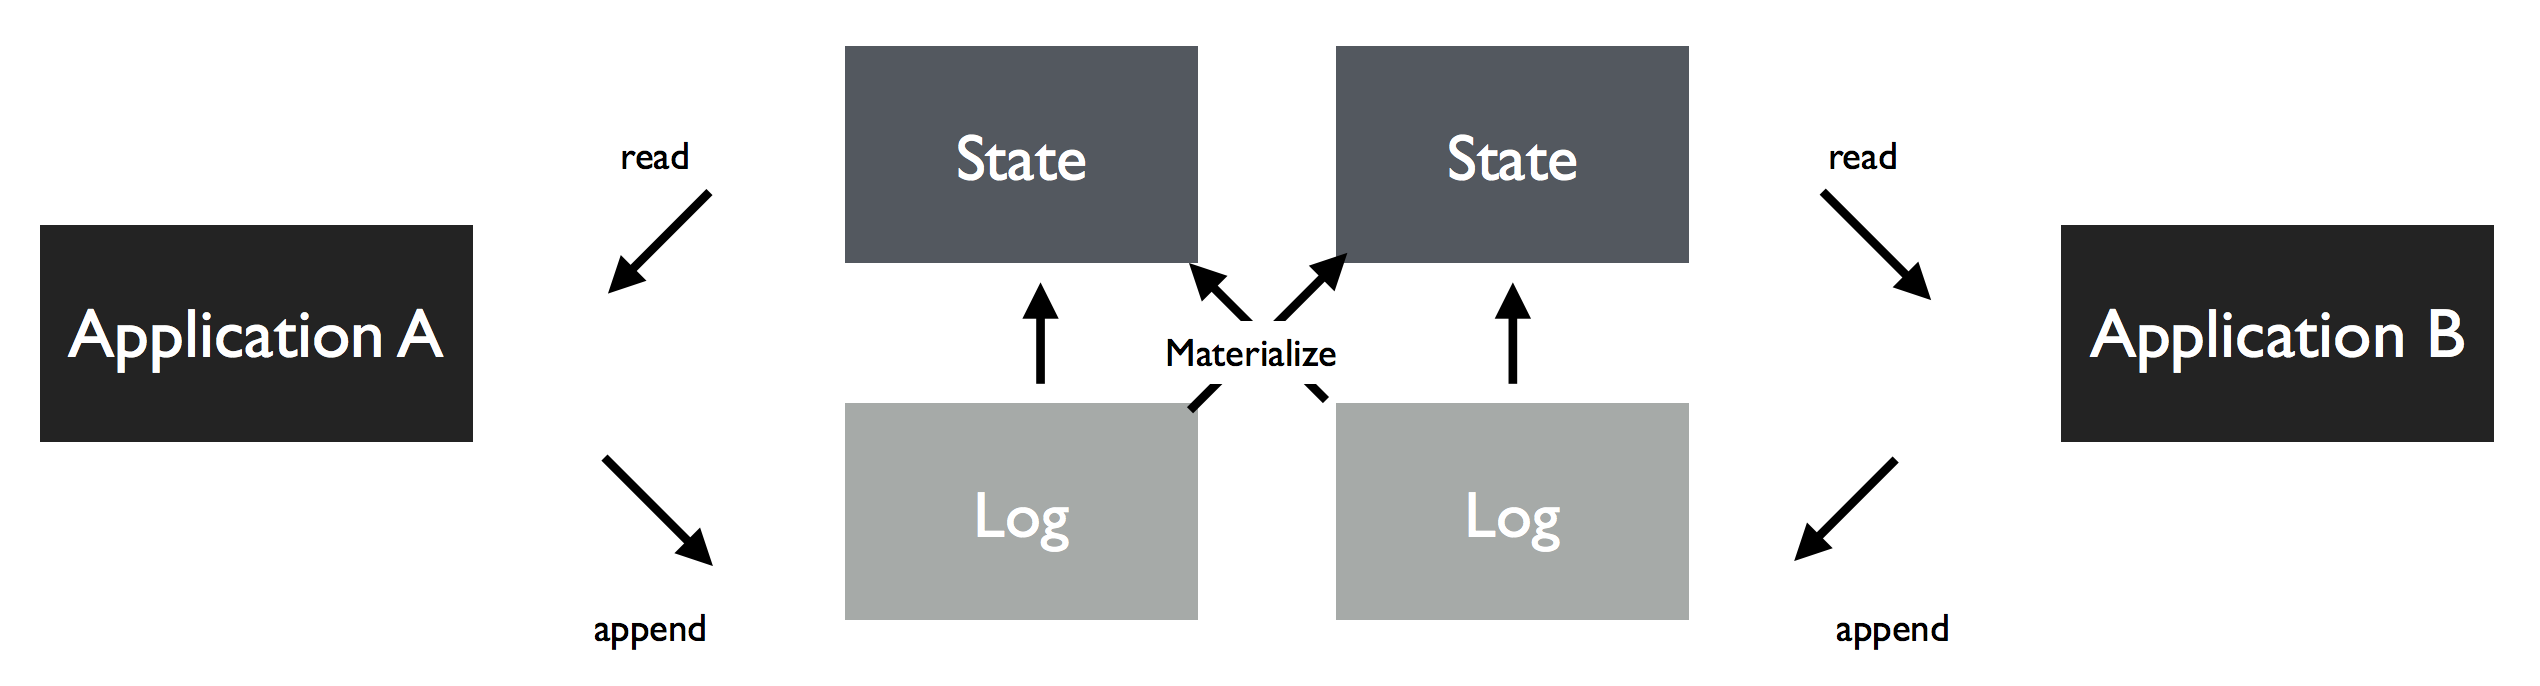
\includegraphics[width=\linewidth]{img/matstate.png}

\subsection{Lambda architecture}
Nathan Marz came up with the term Lambda Architecture (LA) for a generic, scalable and fault-tolerant data processing architecture, based on his experience working on distributed data processing systems at Backtype and Twitter.

The LA aims to satisfy the needs for a robust system that is fault-tolerant, both against hardware failures and human mistakes, being able to serve a wide range of workloads and use cases, and in which low-latency reads and updates are required. The resulting system should be linearly scalable, and it should scale out rather than up.

Here’s how it looks like, from a high-level perspective:

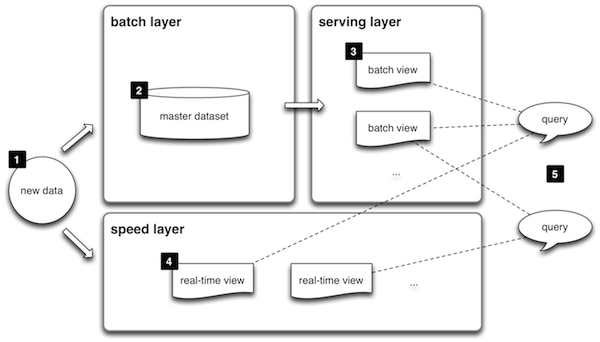
\includegraphics[width=\linewidth]{img/la-arch.png}

\begin{itemize}
\item 1. All data entering the system is dispatched to both the batch layer and the speed layer for processing.
\item 2. The batch layer has two functions: (i) managing the master dataset (an immutable, append-only set of raw data), and (ii) to pre-compute the batch views.
\item 3. The serving layer indexes the batch views so that they can be queried in low-latency, ad-hoc way.
\item 4. The speed layer compensates for the high latency of updates to the serving layer and deals with recent data only.
\item 5. Any incoming query can be answered by merging results from batch views and real-time views.
\end{itemize}

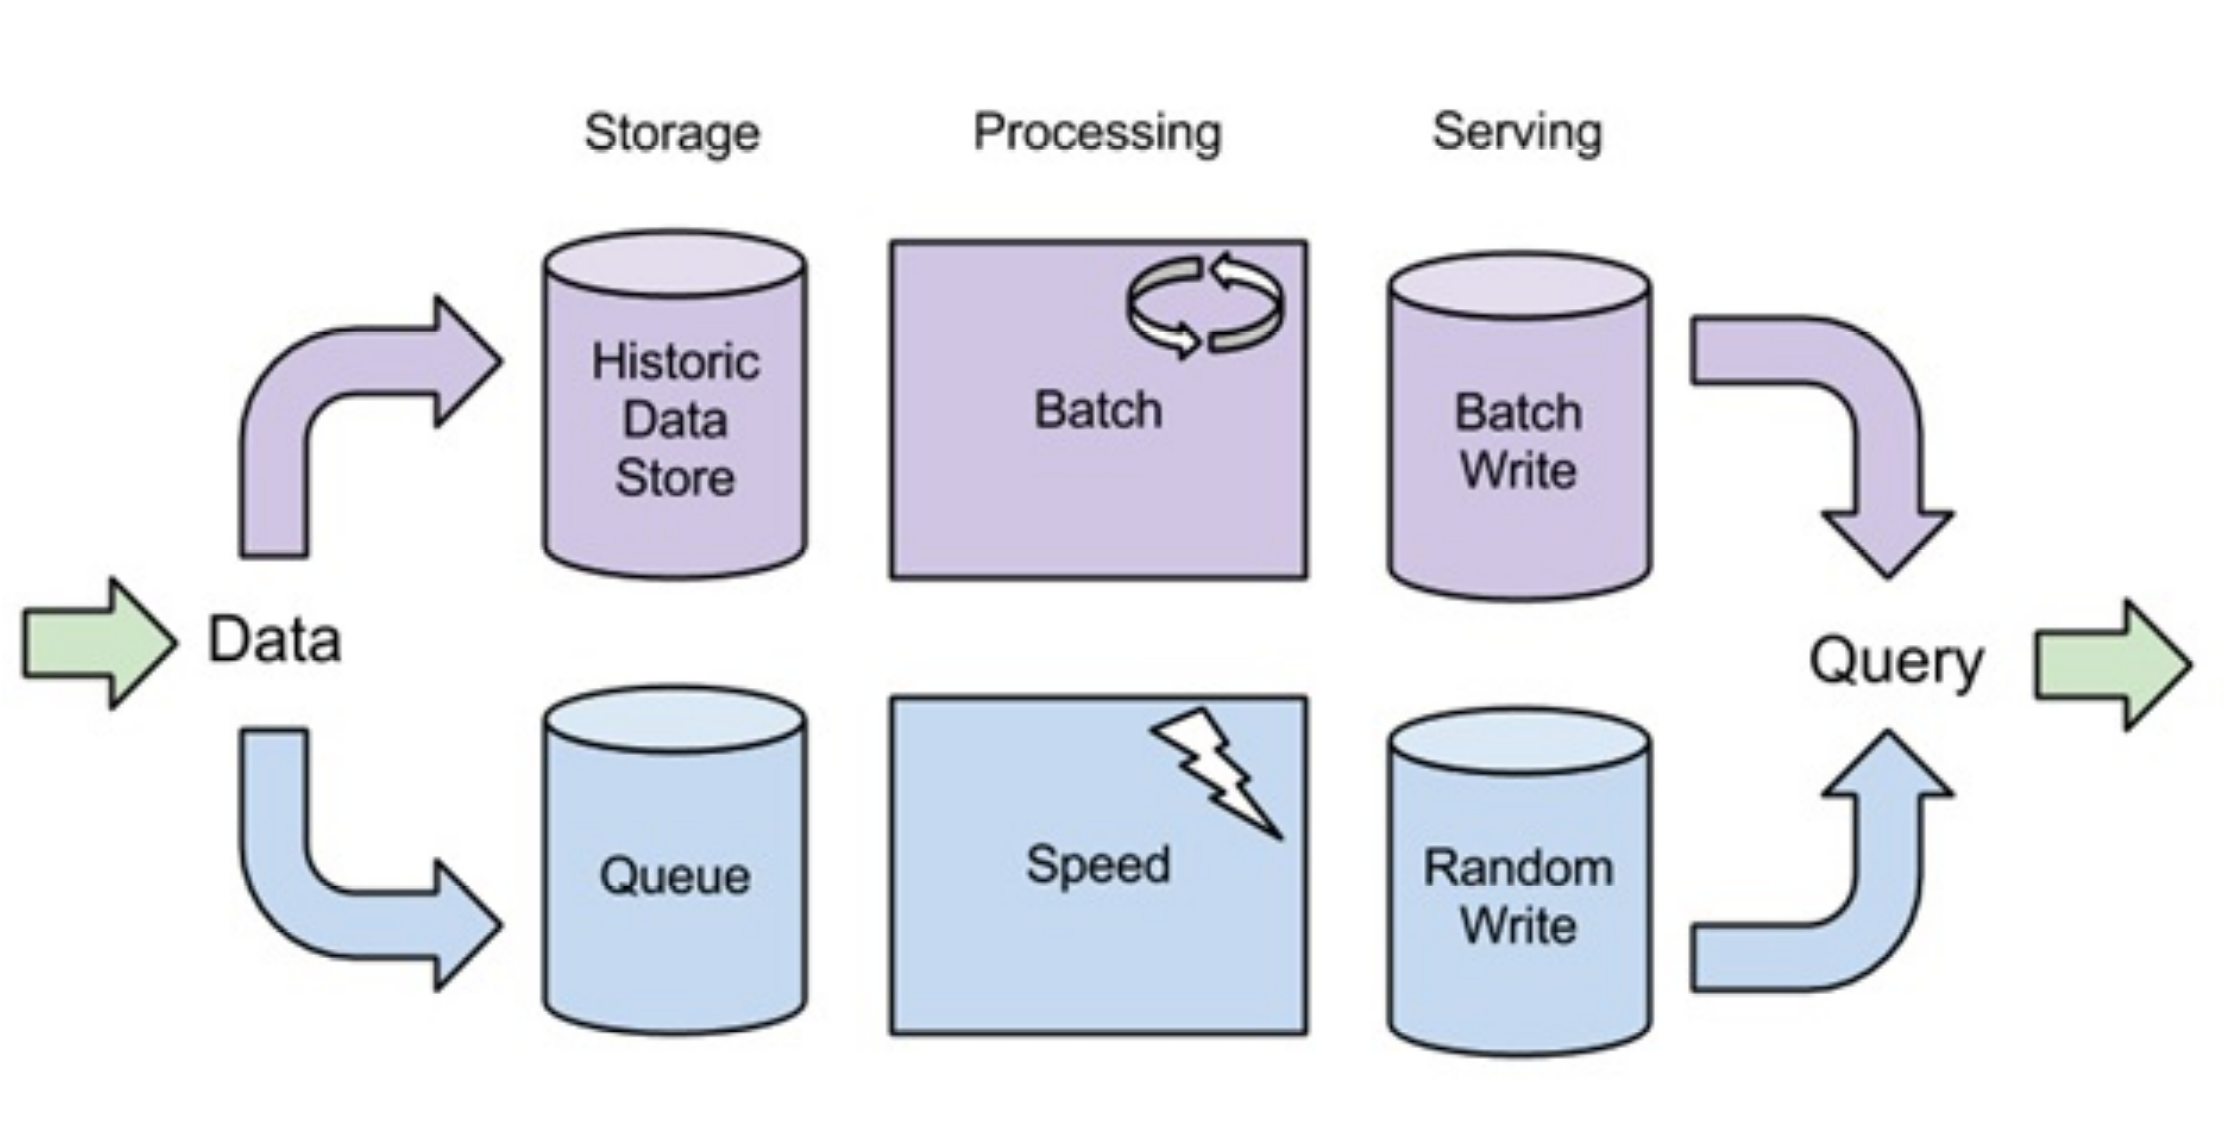
\includegraphics[width=\linewidth]{img/la-2.png}

\subsection{open questions} 
Ad blocker. ID of devices.

\subsection{Cloud Computing}
Commodity Computation, outsourced infrastructure and ability of scaling down and up on demand.


